\documentclass[conference]{IEEEconf}

\input epsf
\usepackage{graphicx}
\usepackage{multirow}
\usepackage{amsmath}
\usepackage{amsfonts}
\usepackage{amssymb}
\renewcommand\thesection{\arabic{section}} % arabic numerals for the sections

\renewcommand\thesubsectiondis{\thesection.\arabic{subsection}.}% arabic numerals for the subsections

\renewcommand\thesubsubsectiondis{\thesubsectiondis.\arabic{subsubsection}.}% arabic numerals for the subsubsections


% correct bad hyphenation here
\hyphenation{28th IEEE Pacific Rim International Symposium on Dependable Computing (PRDC 2023)}
\begin{document}

\title{\textbf{\Large Reliability Analysis of a Mission-critical System via Deep Learning}}

\author{Yan Jiawen, Tadashi Dohi$^{*}$, and Hiroyuki Okamura\\
	\normalsize Graduate School of Advanced Science and Engineering, Hiroshima University, Higashi-Hiroshima 739-8527, Japan\\
	\normalsize \{m220641, dohi, okamu\}@hiroshima-u.ac.jp\\
	\normalsize *corresponding author
}
%+++++++++++++++++++++++++++++++++++++++++++

% use only for invited papers
%\specialpapernotice{(Regular Paper)}

% make the title area
\maketitle
\begin{abstract}

This electronic document is a “live” template. The various components of your paper [title, text, heads, etc.] are already defined on the style sheet, as illustrated by the portions given in this document. DO NOT USE SPECIAL CHARACTERS, SYMBOLS, OR MATH IN YOUR TITLE OR ABSTRACT.This electronic document is a “live” template. The various components of your paper [title, text, heads, etc.] are already defined on the style sheet, as illustrated by the portions given in this document. DO NOT USE SPECIAL CHARACTERS, SYMBOLS, OR MATH IN YOUR TITLE OR ABSTRACT.
\end{abstract}

\IEEEoverridecommandlockouts
\vspace{1.5ex}
\begin{keywords}
mission-critical system; deep learning; censored data; covariate; reliability analysis
\end{keywords}
% no keywords

% For peer review papers, you can put extra information on the cover
% page as needed:
% \begin{center} \bfseries EDICS Category: 3-BBND \end{center}
%
% for peerreview papers, inserts a page break and creates the second title.
% Will be ignored for other modes.
\IEEEpeerreviewmaketitle


%%%%% Section 1 %%%%%
\section{Introduction (Heading 1)} 

Survival analysis provides a statistical method and tool that helps researchers and decision-makers make accurate predictions and wise decisions in various fields. It is important for evaluating treatment effectiveness, predicting survival time, identifying prognostic factors, comparing population survival differences, and assessing reliability and risk. In this article, we studied the application of machine learning in the field of survival analysis. In previous survival analysis methods[1], we often applied them to medical fields, such as clinical trials, epidemiology, cancer research, etc. In this study, we mainly focus on the performance of a deep learning multitasking neural network, DeepHit, in single risk mechanical systems. To compare the effectiveness, we also used other traditional survival analysis methods and machine learning methods, and compared their performance in the fields of medicine and mechanical systems, respectively. In the field of survival analysis, traditional models such as Kaplan Meier and Cox Based Model have problems with low accuracy or inability to consider multiple covariates. Although many machine learning methods can improve accuracy, they cannot effectively handle deleted data in survival analysis. Commonly used machine learning methods include Random Survival Forest, etc. 

%%%%% Section 2 %%%%%
\section{Survival Analysis}

%%%%% 2.1 %%%%%
\subsection{Survival Data with Censoring}

During we analyze survival data, because the observable time will be very limited, the event of interest can not always be observable for us. A conception named censoring was proposed[2].  There are three kinds of censoring:(i)right-censoring: the survival time is longer than the time we can observe.(ii)left-censoring:the survival time is shorter than the time we can observe, but we can not observe the instance any more.(iii)interval censoring: we only can know whether the instance is censored in an interval censoring.In this paper we will focus on right-censoring, because Right-censoring is the most common case. Note that no matter which kind of censoring type, the true censoring time can not be known.
For any survival data, it contains time to event of interest$(S)$ or censoring time$(C)$, if the time to event of interest is longer than the time we can observe, we take censoring time$(C)$ as observe time$(T)$. Otherwise, we use the true time to event of interest$(S)$ as observe time$(T)$. It can be summarized as a formula: $T = min(C,S)$. In this paper we also take the coveriates of every instance into account, for instance i, a triplet can be presented as  $(X_{i},T_{i},\delta_{i})$ , where $X\in R^{1\times N}$ is a feature vector, $\delta_{i}$ is an indicator function, if the instance is right-censoring $\delta_{i} = 0$, or the time to event of interest is known, then $\delta_{i} = 1$.$T_{i}$ denotes the survival time or the right-censoring time, here is the formula:
\begin{eqnarray}
	T_{i} = \begin{cases}
		S_{i} &\text{if } \delta_{i} = 1 \\
		C_{i} &\text{if } \delta_{i} = 0
	\end{cases}
\end{eqnarray}
\subsection{Problem Definition}
The main purpose for survival analysis is to estimate the probability of event occurrence at any time by using survival data witch may have censoring data. The survival function, which is used to represent the probability that the time to the event of interest is not earlier than a specified time t (Lee and Wang 2003; Klein and Moeschberger 2005), which is given as follows:
\begin{eqnarray}
	S(t|X) = Pr\left \{T\ge t|X\right \}
\end{eqnarray}
During $T$ tends to infinity, the survival function must tend to zero. In other words, we believe that when $T=0$, no event of interest has occurred in all instances, but the probability of the event of interest is monotonically increasing with time, and the event will absolutely occur in infinite time. Survival function is decreasing monotonically with time, when $T=0$ survival function equals to 1, which means all the instances are survival. The Survival function represents the probability that the event will not occur after time t. On the contrary, because what we want to know is the probability of the event of interest occurring at Time $T$, cumulative death distribution function $F(t)$ is proposed, if we want to know the probability of the event occurring conveniently before time t, we need to use the following formula as cumulative death distribution function:
\begin{eqnarray}
	F(t|X) = 1 - S(t|X)
\end{eqnarray}

%%%%% 2.2 %%%%%
\subsection{Logistic Regression}

Logistic regression is a statistical method used for modeling and predicting binary classification problems. Let's assume we have a binary dependent variable, denoted as $y$, which takes values 0 or 1. We also have a set of independent variables (or features), denoted as $\mathbf{x} = (x_1, x_2, \ldots, x_n)$, which are used to predict the dependent variable.

Logistic regression transforms the linear combination of the independent variables into a probability value using a logistic function (also known as a sigmoid function). The logistic function is defined as:
\begin{eqnarray}
	g(z) = \frac{1}{1 + e^{-z}}
\end{eqnarray}
Here, $z = \beta_0 + \beta_1x_1 + \beta_2x_2 + \ldots + \beta_nx_n$ represents the linear combination of the independent variables, and $\beta_0, \beta_1, \ldots, \beta_n$ are the regression coefficients.

By applying the logistic function, we can obtain the probability $p(y = 1|\mathbf{x})$ of a sample belonging to class 1:
\begin{eqnarray}
p(y = 1|\mathbf{x}) = g(\mathbf{x} \cdot \boldsymbol{\beta}) = \frac{1}{1 + e^{-(\beta_0 + \beta_1x_1 + \beta_2x_2 + \ldots + \beta_nx_n)}}
\end{eqnarray}
Similarly, we can calculate the probability $p(y = 0|\mathbf{x})$ of a sample belonging to class 0:
\begin{eqnarray}
p(y = 0|\mathbf{x}) = 1 - p(y = 1|\mathbf{x}) = 1 - g(\mathbf{x} \cdot \boldsymbol{\beta})
\end{eqnarray}
Based on the principles of probability theory, we can construct the likelihood function of the logistic regression model using these probabilities. Let's assume we have m training samples denoted as $(\mathbf{x}^{(1)}, y^{(1)}), (\mathbf{x}^{(2)}, y^{(2)}), \ldots, (\mathbf{x}^{(m)}, y^{(m)})$, where $\mathbf{x}^{(i)}$ represents the feature vector of the i-th sample, and $y^{(i)}$ represents the corresponding label.
The likelihood function of the logistic regression model is defined as:
\begin{eqnarray}
	\begin{aligned}
	L(\boldsymbol{\beta}) & = \prod_{i=1}^{m} p(y^{(i)}|\mathbf{x}^{(i)}) 
	\\& = \prod_{i=1}^{m} \left[ (g(\mathbf{x}^{(i)} \cdot \boldsymbol{\beta}))^{y^{(i)}} (1 - g(\mathbf{x}^{(i)} \cdot \boldsymbol{\beta}))^{1-y^{(i)}} \right]
	\end{aligned}
\end{eqnarray}
Our goal is to maximize the likelihood function $L(\boldsymbol{\beta})$, which means finding the regression coefficients $\boldsymbol{\beta}$ that maximize the probability of observing the given data. To facilitate computations, the logarithm of the likelihood function (log-likelihood) is often used instead:
\begin{equation}
\begin{split}
	\log L(\boldsymbol{\beta}) = \sum_{i=1}^{m} [y^{(i)} \log(g(\mathbf{x}^{(i)} \cdot \boldsymbol{\beta})) \\
	+ (1-y^{(i)}) \log(1 - g(\mathbf{x}^{(i)} \cdot \boldsymbol{\beta}))]
\end{split}
\end{equation}
Our objective is to find the regression coefficients $\boldsymbol{\beta}$ that maximize the log-likelihood function $\ell(\boldsymbol{\beta})$. Optimization algorithms such as gradient descent are commonly employed to maximize the log-likelihood function and obtain the best estimates for the regression coefficients.\\

%%%%% 2.3 %%%%%
\subsection{Proportional Hazard Model}

The COX model[4], also known as the Cox proportional hazards model, is a survival analysis method proposed by statistician David Cox in 1972. It is used to examine the relationship between the occurrence time of events (such as death, unemployment, disease recurrence) and multiple predictive factors.

Based on the proportional hazards assumption, the COX model[5] assumes that the risk ratios of the various factors remain constant for event occurrence. This assumption means that if a factor has a risk ratio of 2, then throughout the study period, the risk of event occurrence associated with that factor is always twice that of the other factors. The COX model estimates the risk ratios to describe the impact of the predictive factors on the event occurrence time.The basic form of the COX model is as follows:
\begin{eqnarray}
	h(t) = h_{0}(t) * exp(b_{1}x_{1} + b_{2}x_{2} + ... + b_{p}x_{p})
\end{eqnarray}
Here, h(t) represents the risk (i.e., the rate of event occurrence) at time t, h0(t) is the baseline hazard function (or baseline hazard curve), $[x_{1}, x_{2}, ..., x_{p}]$ are the values of the predictive factors, and  $[b_{1}, b_{2}, ..., b_{p}]$  are the corresponding regression coefficients.
Here if we want to know the survival function, we can use this formula:
\begin{eqnarray}
	S(t)=exp(-\int_{0}^{t}h(u)du )
\end{eqnarray}
One of the advantages of the COX model is that it does not require assumptions about the distribution of event occurrence times, making it suitable for various types of data. Additionally, the COX model can consider the complex effects of multiple factors on event occurrence, not just the effect of a single factor. It can also handle truncated data, which occur when events are observed before or after a specific time point.

To estimate the parameters of the COX model, a common approach is to use partial likelihood estimation. By maximizing the partial likelihood function, estimates of the regression coefficients can be obtained. Hypothesis testing can also be performed to assess the significance of the predictive factors.

%%%%% 2.4 %%%%%
\subsection{Random Survival Forest}

Random Survival Forest [9] A Random Survival Forest is a statistical method based on decision trees used for survival analysis and prediction. It combines the concepts of random forests and survival analysis to handle data with time-to-event information.Random Survival Forest involves constructing multiple decision trees for prediction and analysis. Each decision tree is built using randomly sampled data and a subset of features to increase model diversity and reduce the risk of overfitting. The random sampling process is typically performed using bootstrapping.

For each decision tree, at each node, a random survival forest selects a feature and corresponding split point based on a splitting criterion (e.g., Log-Rank statistic). This process is performed to maximize the splitting gain at each node. Ultimately, the predictions from all the decision trees are combined to obtain the overall prediction of the random survival forest.In a random survival forest, the prediction target is the survival function or survival curve. Typically, survival functions are represented using Kaplan-Meier curves, survival probabilities, or hazard ratios. Suppose we have a random survival forest model denoted as $\mathcal{F}$, given an input sample $\mathbf{X}$, the model's predicted output is the estimated survival function $\hat{S}(t)$. The prediction of the random survival forest can be represented as:

\begin{equation}
	\hat{S}(t) = \frac{1}{B} \sum_{b=1}^B \hat{S}_b(t)
\end{equation}

Here, $B$ represents the number of decision trees, and $\hat{S}_b(t)$ is the survival function prediction of the $b$-th decision tree.

A random survival forest model can be used for predicting individual survival probabilities, assessing feature importance, and identifying factors that affect survival. It is widely applied in medical research, biostatistics, and other fields, especially for handling complex survival data and large-scale datasets

%%%%% Section 3 %%%%%
\section{Deep Leaning}

%%%%% 3.1 %%%%%
\subsection{Deephit}

DeepHit[3] is a multi-task network and the network structure is different form conventional multi-task network. Deephit use single softmax layer as the output layer, a shared sub-network and  $K=[\varnothing,1,2,3,...,K]$ cause-specific sub-networks are used to consist the multi-task function. Lee. el at utilize the single softmax as the output layer of DeepHit in order to learn the joint distribution of $K$ competing events not the marginal of each event, and a residual connection is maintained from the input coveriates into the input covariates into the input of each cause-specific sub-network.
\begin{figure}[htbp]
	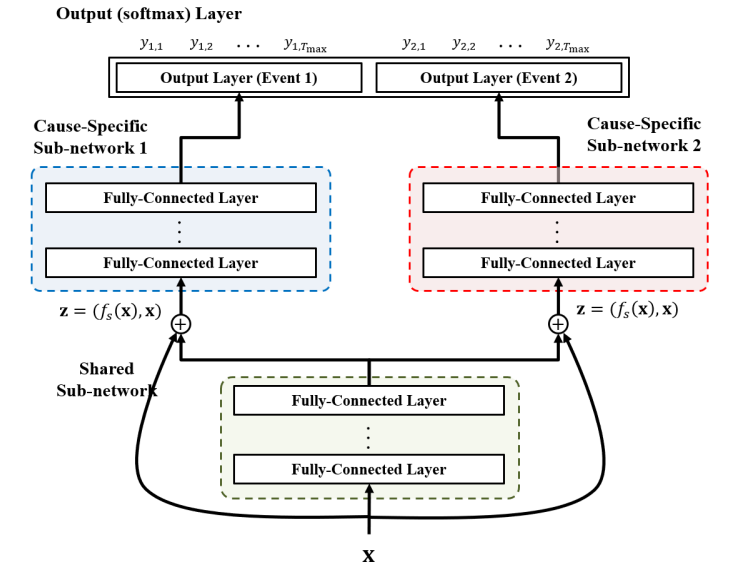
\includegraphics[scale=0.5]{network.jpg}
	\caption{DeeHit network structure}
\end{figure}
DeepHit designs a shared sub-network and K use-specific sub-networks for $K$ competing risk events. Each use-specific sub-network consists of two fully connected layers, $L_{s}$ and $L_{c,k},k\in K$, respectively. The shared sub-network takes the input of covariates $x$ and outputs a vector $f_{s}(x)$ containing potential features for K competing events. To address the competing risk problem, each cause-specific sub-network receives a vector $f_{c,k}(z)$ as input, where $f_{c,k}(z)$ is composed of the output $f_{s}(x)$ from the shared sub-network and the input covariates x, and outputs fz(x) as the probability of event k occurring at time t. Specifically, the output $f_{s}(x)$ of the shared sub-network is combined with the covariates $X$ vector, allowing the cause-specific sub-network to simultaneously extract the common and unique parts of $f_{s}(x)$ and $X$ features. Learning only $f_{s}(x)$may result in the loss of the unique parts. The sum of the outputs of all cause-specific sub-networks represents the first-hit event and the joint probability distribution of events, requiring cause-specific sub-networks to learn the probability distribution of the first-hit time for each cause in parallel. The output layer uses softmax, and its output $y=[y_{1,1}, y_{1,2},...,y_{k,T_{max}}]$ represents the instantaneous occurrence probabilities of the events of interest at each time point. For example, for patient i with covariates Xi, the instantaneous probability of event k=1 occurring at time $t$, $y_{k,t}$, is given by $\hat{P}(s, k|X_{i})$.
The (cause-specific) cumulative incidence function(CIF) for instance $i$ and event $k_{i}\in K$:
\begin{eqnarray}
	\begin{aligned}
		F_{k_{i}}(t_{i}|x_{i}) = P\left(s<t_{i},k=k_{i}|x=x_{i}\right) \\
		= \sum_{t^*=0}^{t_{i}} P\left(t=t^*,k=k_{i}|x=x_{i}\right)
	\end{aligned}
\end{eqnarray}
CIF presents the probability that the $k_{i} \in K$ occurs on or before time $t_{i}$ conditional on covariates $x_{i}$. The true CIF never can be known for us, we use 	$F_{k_{i}}(t_{i}|x_{i}) = \sum_{m=0}^{t_{i}}y_{k,t}$, in order to compare the risk of event occuring and to assess how models discriminate across cause -specific risks among patients.

A total loss function, denoted as $L_{total}$, is defined to train DeepHit, . By minimizing this loss function, we can optimize the model. $L_{total}$ consists of two components: $L_{1}$, which is derived from the joint probability distribution of the first hitting time, and $L_{2}$, which is a loss function that ranks the events of interest in the presence of competing risks.And $L_{total}$ is given by this formula:
\begin{eqnarray}
	L_{total} = L_{1}+L_{2}
\end{eqnarray}

$L_{1}$ represents the likelihood function of the joint probability distribution of the first hitting time for the corresponding event. For instances without censoring, $L_{1}$ takes into account both the event type that has occurred and the time of event occurrence. For censored instances, it captures information up until the censoring time.In other words, $L_{1}$ considers the observed events and their corresponding times, as well as the censored instances where the exact event time is unknown but information up until the censoring time is available. By incorporating all these aspects, $L_{1}$ captures the information related to the occurrence of events and the time to event.$L_{1}$ is defined as follow:
\begin{eqnarray}
	\begin{aligned}
	L_{1}=-\sum_{i=1}^{N}\left[\mathbb{I}\left(k^{(i)} \neq \varnothing\right) \cdot \log \left(y_{k^{(i)}, t^{(i)}}^{(i)}\right)\right. \\
	\left.+\mathbb{I}\left(k^{(i)}=\varnothing\right) \cdot \log \left(1-\sum_{k=1}^{K} \hat{F}_{k}\left(t^{(i)} \mid \mathbf{x}^{(i)}\right)\right)\right]
\end{aligned}
\end{eqnarray}
where $\mathbb{I}(\cdot)$ is an indicator function.The $L_{1}$ term captures all the information from uncensored instances up until the occurrence of the event of interest, while the second term captures all the information from censored instances at the right-censoring time. To fine-tune each cause-specific sub-network, DeepHit introduces $L_{2}$ to merge all the estimated cumulative incidence functions (CIF) at different times. In this context, DeepHit utilizes a ranking loss function (Harrel et al., 1982), which is based on the core idea that an instance experiencing the event of interest at time s must have a higher risk than instances that are still alive at time s.Define:
\begin{eqnarray}
	R_{k,i,j}=\mathbb{I}(k^{(i)}=k,s^{(i)}<s^{(j)}) 
\end{eqnarray}
for the indicator function of pairs $(i,j)$ who experience risk $k$ at different time, and the risk for event $k$ can be directly compared, these pair is called acceptable for event $k$.Now define:
\begin{eqnarray}
	L_{2}=\sum_{k=1}^{K}\alpha_{k}\sum_{i \ne j}^{}R_{k,i,j}\eta\left(\hat{F}_{k}(t^{(i)}|x^{(i)}),\hat{F}_{k}(t^{(i)}|x^{(j)})\right)
\end{eqnarray}
The coefficient $\alpha_{k}$ are chosen to trade off the $k$-th competing event, and $\eta(x,y)=exp(\frac{-(x-y)}{\sigma})$ is a convex loss function, which incorporating $L_{2}$ into the total loss function penalizes incorrect ordering of pairs respectively to each event and minimizing the total loss encourages correct ordering of pairs respectively to each event. 

%%%%% Section 4 %%%%%
\section{Experiment}

%%%%% 4.1 %%%%%
\subsection{Data Set}

\textbf{METABRIC} The Molecular Taxonomy of Breast Cancer International Consortium(METABRIC) dataset contains gene expression profiles and clinical features. The dataset consists of 1982 patients, 888 patients($44.8\%$) were observed until their death, and the remaining 1093 patients($55.2\%$) were censored.

To analyze the dataset, we focus on 21 clinical features which include information such as tumor size, the number of positive lymph nodes,and other relevant factors, for more details see(Bilal et al. 2013). To handle missing values, for real-valued features we used the mean-value to replace it. And 	One-hot encoding was applied for categorical features.
\\

\textbf{NTJE} The NASA Turbofan Jet Engine dataset (NTJE) contains information about engine operational settings, sensor measurements, and failure time of jet engines. Among the recorded variables, there are 3 operational settings and 26 sensor measurements available for analysis. However, for our specific analysis, we narrow our focus to 2 operational settings and 8 sensor measurements based on a correlation analysis.

To simulate censored data, we assume that the devices were observed until a specific time point, which is 200 units of time. The dataset consists of a total of 708 devices, out of which 331 ($46.8\%$) were observed until they experienced failure. The remaining 377 devices ($53.2\%$) were right-censored, meaning their failure times were not observed within the given observation period.

To evaluate the application of various models on the dataset, we randomly divide the dataset into a training set ($80\%$) and a test set ($20\%$). Additionally, we reserve $20\%$ of the training set as a validation set, ensuring that the proportion of missing data to complete data is consistent across these datasets. The parameters $\alpha$ and $\sigma$ in $L_{total}$ are determined based on the discriminative performance on the validation set. We employ early stopping based on the total loss. DeepHit is a 4-layer network model consisting of one fully connected layer serving as the shared sub-network, two fully connected layers serving as cause-specific sub-networks, and one softmax layer as the output layer. The number of nodes in the hidden layers is determined based on the covariate dimension, with 3, 5, and 3 times the covariate dimension used as the number of nodes for the first, second, and third hidden layers, respectively. In the backpropagation process, we utilize the Adam optimizer with a batch size of 32, a learning rate of $10^{-4}$, and a dropout probability of 0.65. Xavier initialization is applied to all layers.For other models, we also fine-tune the models by find the best performance point.

%%%%% 4.2 %%%%%
\subsection{Benchmark}

\textbf{C-index}[6] When evaluating the performance of a classification model, one commonly used metric is the C-index (also known as the Concordance Index, Concordance Probability Estimate, or Concordance Discrimination Index). The C-index is a measure of the model's ability to correctly rank samples, and it is widely applied in the field of survival analysis.

The calculation of the C-index is based on comparing the predicted probabilities of the model with the actual observed outcomes. It can be used to evaluate any binary classification model, but in survival analysis, it is often used to assess models that predict survival times, such as survival regression models.

The C-index[7] ranges from 0.5 to 1, where 0.5 indicates that the model's predicted rankings are completely unrelated to the actual observed rankings, and 1 indicates that the model perfectly predicts the sample rankings. In other words, a higher C-index indicates better model performance.
There are several ways to calcuting the C-index:
(i)If the output of the model is a hazard ratio, such as Cox based model, C-index is give by the formula: 
\begin{eqnarray}
	\hat{C}=\frac{1}{num}\sum_{i:\delta_{i}}^{}\sum_{j:y_{i}<y_{j}}^{}\mathbb{I}[X_{i}\hat{\theta}>X_{j}\hat{\theta}]
\end{eqnarray}
where $i,j\in{1,2,...,N}$, $num$ denotes the number of all comparable pairs, $\mathbb{I}[\cdot]$ is the indicator function, and $\hat{\theta}$ is estimated parameters from the Cox based models.
(ii) For survival methods which aim to directly learn the survival time, the C-index is given by this:
\begin{eqnarray}
	\hat{C}=\frac{1}{num}\sum_{i:\delta_{i}}^{}\sum_{j:y_{i}<y_{j}}^{}\mathbb{I}[S(\hat{y_{i}|X_{j}})>S(\hat{y_{i}}|X_{j})>\hat{y_{i}}|X_{i})]
\end{eqnarray}
where $S(\cdot)$ estimates the survival probability.\\

\textbf{Brier Score} When evaluating the accuracy of probability prediction models, the Brier Score is a commonly used metric. It takes into account both the correctness of the predictions and the confidence of the probability estimates.

The calculation formula for the Brier Score is:
\begin{eqnarray}
	BS = \frac{1}{N} \sum_{i=1}^{N} (f_i - o_i)^2
\end{eqnarray}
where $N$ represents the number of samples, $f_{i}$ represents the predicted probability for the ith sample, and $o_{i}$ represents the observed outcome for the ith sample.

The computation process of the Brier Score is as follows:

a. For each sample, calculate the difference between the predicted probability fi and the observed outcome oi.\\
b. Square the difference to amplify the prediction error.\\
c. Sum up the squared differences for all samples.\\
d. Divide the sum by the number of samples N to obtain the Brier Score.\\

The Brier Score ranges from $0$ to $1$. A Brier Score of $0$ indicates perfect predictions, while a score of $1$ indicates the worst predictions. Therefore, a lower Brier Score indicates higher prediction accuracy of the model.

%%%%% 4.3 %%%%%
\subsection{Performance Comparison}

Compared to other evaluation metrics, the Brier Score has some advantages. Firstly, it is sensitive to the calibration of predicted probabilities, reflecting the accuracy and reliability of the model's probability estimates. Secondly, the Brier Score remains stable even with a small number of samples and is not affected by extreme prediction results.
\begin{table}[]
	\centering
	\centerline {Table 1. RESULTS}
	\begin{tabular}{|c|cc|cc|}
		\hline
		\multirow{2}{*}{\textbf{models}} & \multicolumn{2}{c|}{\textbf{METABRIC}}              & \multicolumn{2}{c|}{\textbf{NTJE}}                  \\ \cline{2-5} 
		& \multicolumn{1}{c|}{\textbf{C-index}} & \textbf{BS} & \multicolumn{1}{c|}{\textbf{C-index}} & \textbf{BS} \\ \hline
		\textbf{DEEPHIT}                 & \multicolumn{1}{c|}{0.691}            & 0.055       & \multicolumn{1}{c|}{0.745}            & 0.013       \\ \hline
		\textbf{COX}                     & \multicolumn{1}{c|}{0.640}            & 0.057       & \multicolumn{1}{c|}{0.697}            & 0.023       \\ \hline
		\textbf{Logistic}                & \multicolumn{1}{c|}{0.622}            & 0.346       & \multicolumn{1}{c|}{0.663}            & 0.296       \\ \hline
		\textbf{Adaboost}                & \multicolumn{1}{c|}{0.644}            & 0.227       & \multicolumn{1}{c|}{0.721}            & 0.205       \\ \hline
		\textbf{RSF}                      & \multicolumn{1}{c|}{0.642}            & 0.220       & \multicolumn{1}{c|}{0.713}            & 0.199       \\ \hline
	\end{tabular}
\end{table}

\begin{figure}[htbp]
	\centering
	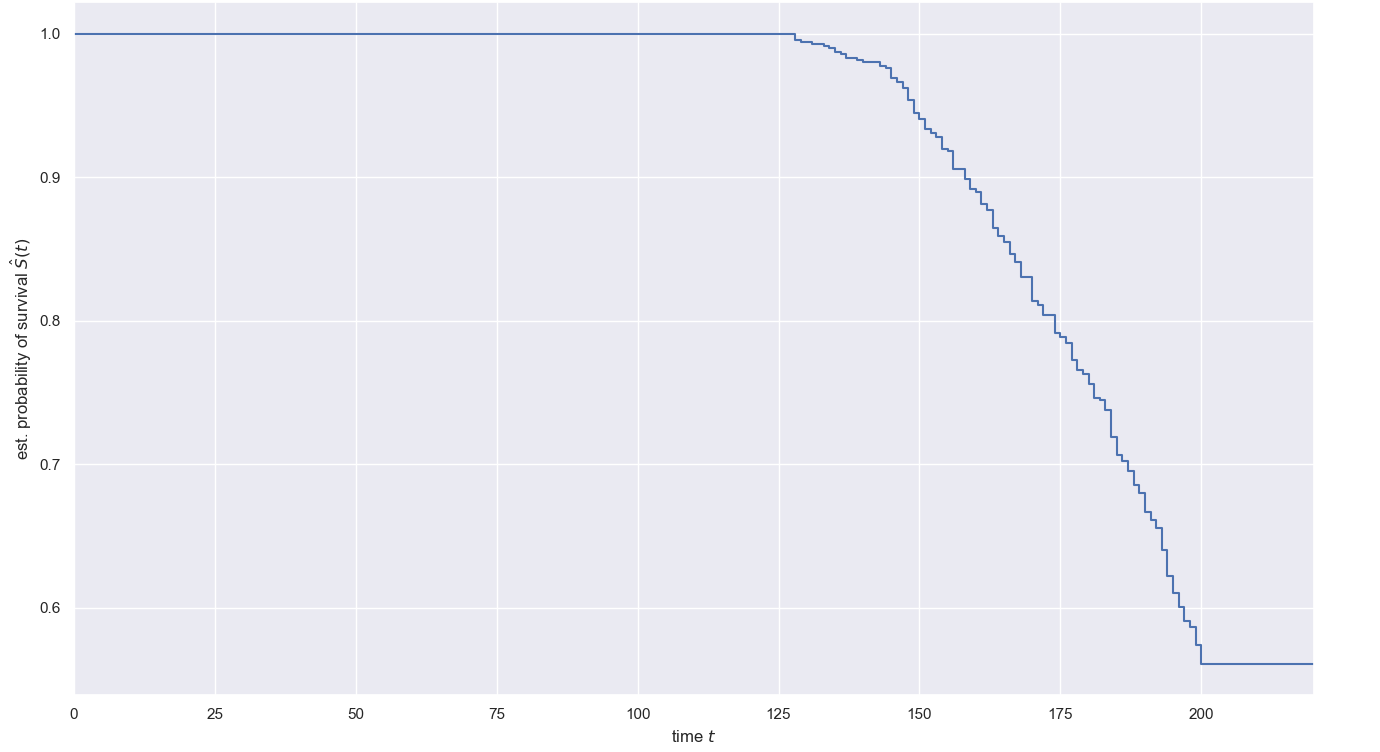
\includegraphics[scale=0.26]{Kaplan_Meier.png}
	\caption{Kaplan Meier Curve}
\end{figure}
\subsection{Result}

%%%%% 4.4 %%%%%
\subsection{Reliability Assessment}

The Kaplan-Meier[7] curve is a non-parametric estimator, meaning that it does not make assumptions about the underlying probability distribution of survival times. Instead, it calculates the survival probability at each observed event time point based on the number of individuals at risk and the number of events that have occurred up to that time point.

The Kaplan-Meier estimator takes into account censoring, which occurs when the event of interest has not occurred for some individuals by the end of the study or they are lost to follow-up. Censoring is indicated in the curve by vertical ticks or lines, indicating that the survival status of those individuals is unknown beyond that point.

The Kaplan-Meier curve[8] is typically plotted as a step function, where the horizontal axis represents time, and the vertical axis represents the estimated survival probability. The curve starts at 1.0 (indicating 100\% survival) at the beginning of the study and decreases as events occur or individuals are censored.

The Kaplan-Meier curve is a graphical tool used in survival analysis to estimate the cumulative distribution function (CDF) of the probability of an event occurring. Below is the LaTeX formula for the Kaplan-Meier curve:

\begin{eqnarray}
S(t) = \prod_{i:t_i \leq t} \left(1 - \frac{d_i}{n_i}\right)
\end{eqnarray}

Here, $S(t)$ represents the proportion of patients surviving until time $t$. $t_i$ denotes the time of occurrence of event $i$, $d_i$ represents the number of events that occur at time $t_i$, and $n_i$ is the number of patients at risk at time $t_i$.

%%%%% Section 5 %%%%%
\section{Conclusion}




% use section* for acknowledgment
%\section*{Acknowledgment}


%%%%%%%%%%
\begin{thebibliography}{1}


\bibitem {ref9}
L. Breiman, Random forests, 
\newblock {\it{Machine Learning}}, vol. 45, no. 1, pp. 5--32, 2001.

\bibitem {ref4}
D. R. Cox R. David, Regression models and life tables, 
\newblock {\it{Journal of the Royal Statistical Society}}, vol. 34, no. 2, pp. 187-–220, 1972.

\bibitem {ref5}
D. R. Cox, Partial likelihood, 
\newblock {\it{Biometrika}}, vol. 62, no. 2, pp. 269-–276, 1975.

\bibitem {ref6}
F. E. Harrell, R. M. Califf, D. B. Pryor, K. L. Lee, and R. A. Rosati, Evaluating the yield of medical tests, 
\newblock {\it{Journal of the American Medical Association}}, vol. 247, no. 18, pp. 2543–-2546, 1982. 

\bibitem {ref7}
F. E. Harrell, K. L. Lee, R. M. Califf, D. B. Pryor, and R. A. Rosati, Regression modelling strategies for improved prognostic prediction, 
\newblock {\it{Statistics in Medicine}}, vol. 3, no. 2, pp. 143-–152, 1984. 

\bibitem {ref8}
E. L. Kaplan and P. Meier, Nonparametric estimation from incomplete observations, 
\newblock {\it{Journal of the American Statistical Association}}, vol. 53, no. 282, pp. 457–-481, 1958. 

\bibitem {ref2}
J. P. Klein, and M. L. Moeschberger, 
{\it{Survival Analysis: Techniques for Censored and Truncated Data}}, Springer, New York, 2003. 

\bibitem {ref3}
C. Lee, W. R. Zame, J. Yoon, M. van der Schaar, DeepHit: A deep learning approach to survival analysis with competing risks, 
\newblock {\it{Proceedings of the AAAI Conference on Artificial Intelligence (AAAI)}}, 2018. 

\bibitem {ref1}
P. Wang, Y.Li, and C. K. Reddy, Machine learning for survival analysis: A survey, 
\newblock {\it{ACM Computing Surveys}}, vol. 51, no. 6, pp. 1--36, 2019

\end{thebibliography}
\end{document}